\documentclass[13pt]{beamer}

\setbeamertemplate{navigation symbols}{}
\defbeamertemplate*{footline}{infolines theme}
{
  \leavevmode%
  \hbox{%
  \begin{beamercolorbox}[wd=.99\paperwidth,ht=2.25ex,dp=1ex,right]{date in head/foot}%
    \usebeamerfont{date in head/foot}\insertshortdate{}
    \hfill
    {\footnotesize {\small \insertframenumber{}}} %/ \inserttotalframenumber\hspace*{2ex}
  \end{beamercolorbox}}%
  \vskip0pt%
}

\hypersetup{colorlinks,linkcolor=blue,citecolor=darkgreen,urlcolor=blue}
\usepackage{tikz}
\usetikzlibrary{fit,shapes,positioning,backgrounds,calc,patterns,scopes,decorations,chains,arrows,matrix,decorations.pathreplacing}
\usepackage{fontspec}
\usepackage{xunicode}
\usepackage{xltxtra}
\defaultfontfeatures{Mapping=tex-text}
%\usepackage[norules,nolineno]{lgrind}
\usepackage{epsf}
\usepackage{color}
\usepackage{bbding} % stars ...
\usepackage{pifont} % stars ...
\usepackage{pstricks}
\usepackage{url}
%\usepackage{calc}
\usepackage{graphicx}
\usepackage{ifthen}
\usepackage{subfigure}
\usepackage{fancyhdr}
\usepackage{multido}
\usepackage{wasysym}
\usepackage{fp}
\usepackage{listings}
\usepackage{amsmath}
\usepackage{array}
\usepackage{multirow}
\usepackage{paralist}
\usepackage{ulem}
\normalem
\lstset{language=C,tabsize=2,basicstyle=\ttfamily\normalsize,backgroundcolor=\color{LemonChiffon},framerule=1pt,frame=single}
\usepackage[noend]{algorithm2e}
\usepackage{verbatim}
\usepackage{skull}

\newenvironment{sItemize}%
  {\begin{list}{-}{\leftmargin=1em\itemsep=0em\parskip=0pt\parsep=-2pt}}%
  {\end{list}}


\definecolor{lightblue}{rgb}{0.68,0.85,0.90}
\definecolor{red3}{rgb}{0.80,0.00,0.00}
\definecolor{darkgreen}{rgb}{0.00,0.39,0.00}
\definecolor{LemonChiffon}{rgb}{1.00,0.98,0.80}
\definecolor{DarkBlue}{rgb}{0.00,0.00,0.55}
\tikzset{c1/.style={ellipse,draw=blue!50,fill=blue!20,ultra thick,minimum size=5mm}}
\tikzset{spawn-n/.style={inner sep=2pt,circle,draw,fill=darkgreen,anchor=center,draw=darkgreen}}
\tikzset{sync-n/.style={inner sep=2pt,circle,draw,fill=red3,anchor=center,draw=red3}}
\tikzset{fn-n/.style={c1,anchor=center,inner sep=2pt,fill=black!60,draw=black,text=white}}
\tikzset{fn-x/.style={c1,anchor=center,inner sep=1pt,fill=black!40,draw=black,text=white,thin}}
\tikzset{fn-g/.style={rectangle,anchor=center,inner sep=5pt,fill=black!20,draw=black,text=white}}
\tikzset{spawn-e/.style={-stealth,very thick,draw=darkgreen,fill=darkgreen}}
\tikzset{sync-e/.style={-stealth,very thick,draw=red3,fill=red3}}
\tikzset{fn-e/.style={-stealth,very thick,draw=black,fill=black}}
\tikzset{note/.style={rectangle, fill=LemonChiffon, thick, draw=DarkBlue,rounded corners=1ex}}
\tikzset{code/.style={rectangle, fill=black!10, draw=black, thick, rounded corners=1ex,text=black, inner sep=4pt}}
\tikzset{cons/.style={rectangle, fill=LemonChiffon, draw=black, thick, rounded corners=1ex,text=black, inner sep=9pt}}

\tikzset{fn-inact/.style={
    rectangle, fill=black!20, thick, draw=black,
    rounded corners=1ex,minimum height=1cm, minimum width=1.3cm
}}

\tikzset{fn-activ/.style={
    rectangle, fill=green!30, thick, draw=black,
    rounded corners=1ex,minimum height=1cm, minimum width=1.3cm
}}

% http://tex.stackexchange.com/questions/16964/block-quote-with-big-quotation-marks
\usepackage{ifxetex}
\ifxetex{%
  \newfontfamily\quotefont[Ligatures=TeX]{Linux Libertine O} % or any font on your system
\else
  \newcommand*\quotefont{\fontfamily{fxl}} % selects Libertine for quote font
\fi

\title{{\LARGE The Implementation of the Cilk-5 Multithreaded Language}\\
       \medskip
       M. Frigo, C. E. Leiserson, K. H. Randall
       \medskip
}
\subtitle{\bigskip\Large{}PWL: Zurich}
\author{Kornilios Kourtis}
\date{27 April, 2017}

\begin{document}
\maketitle

\begin{frame}{Previously on PWL: Zurich}
	\begin{center}
	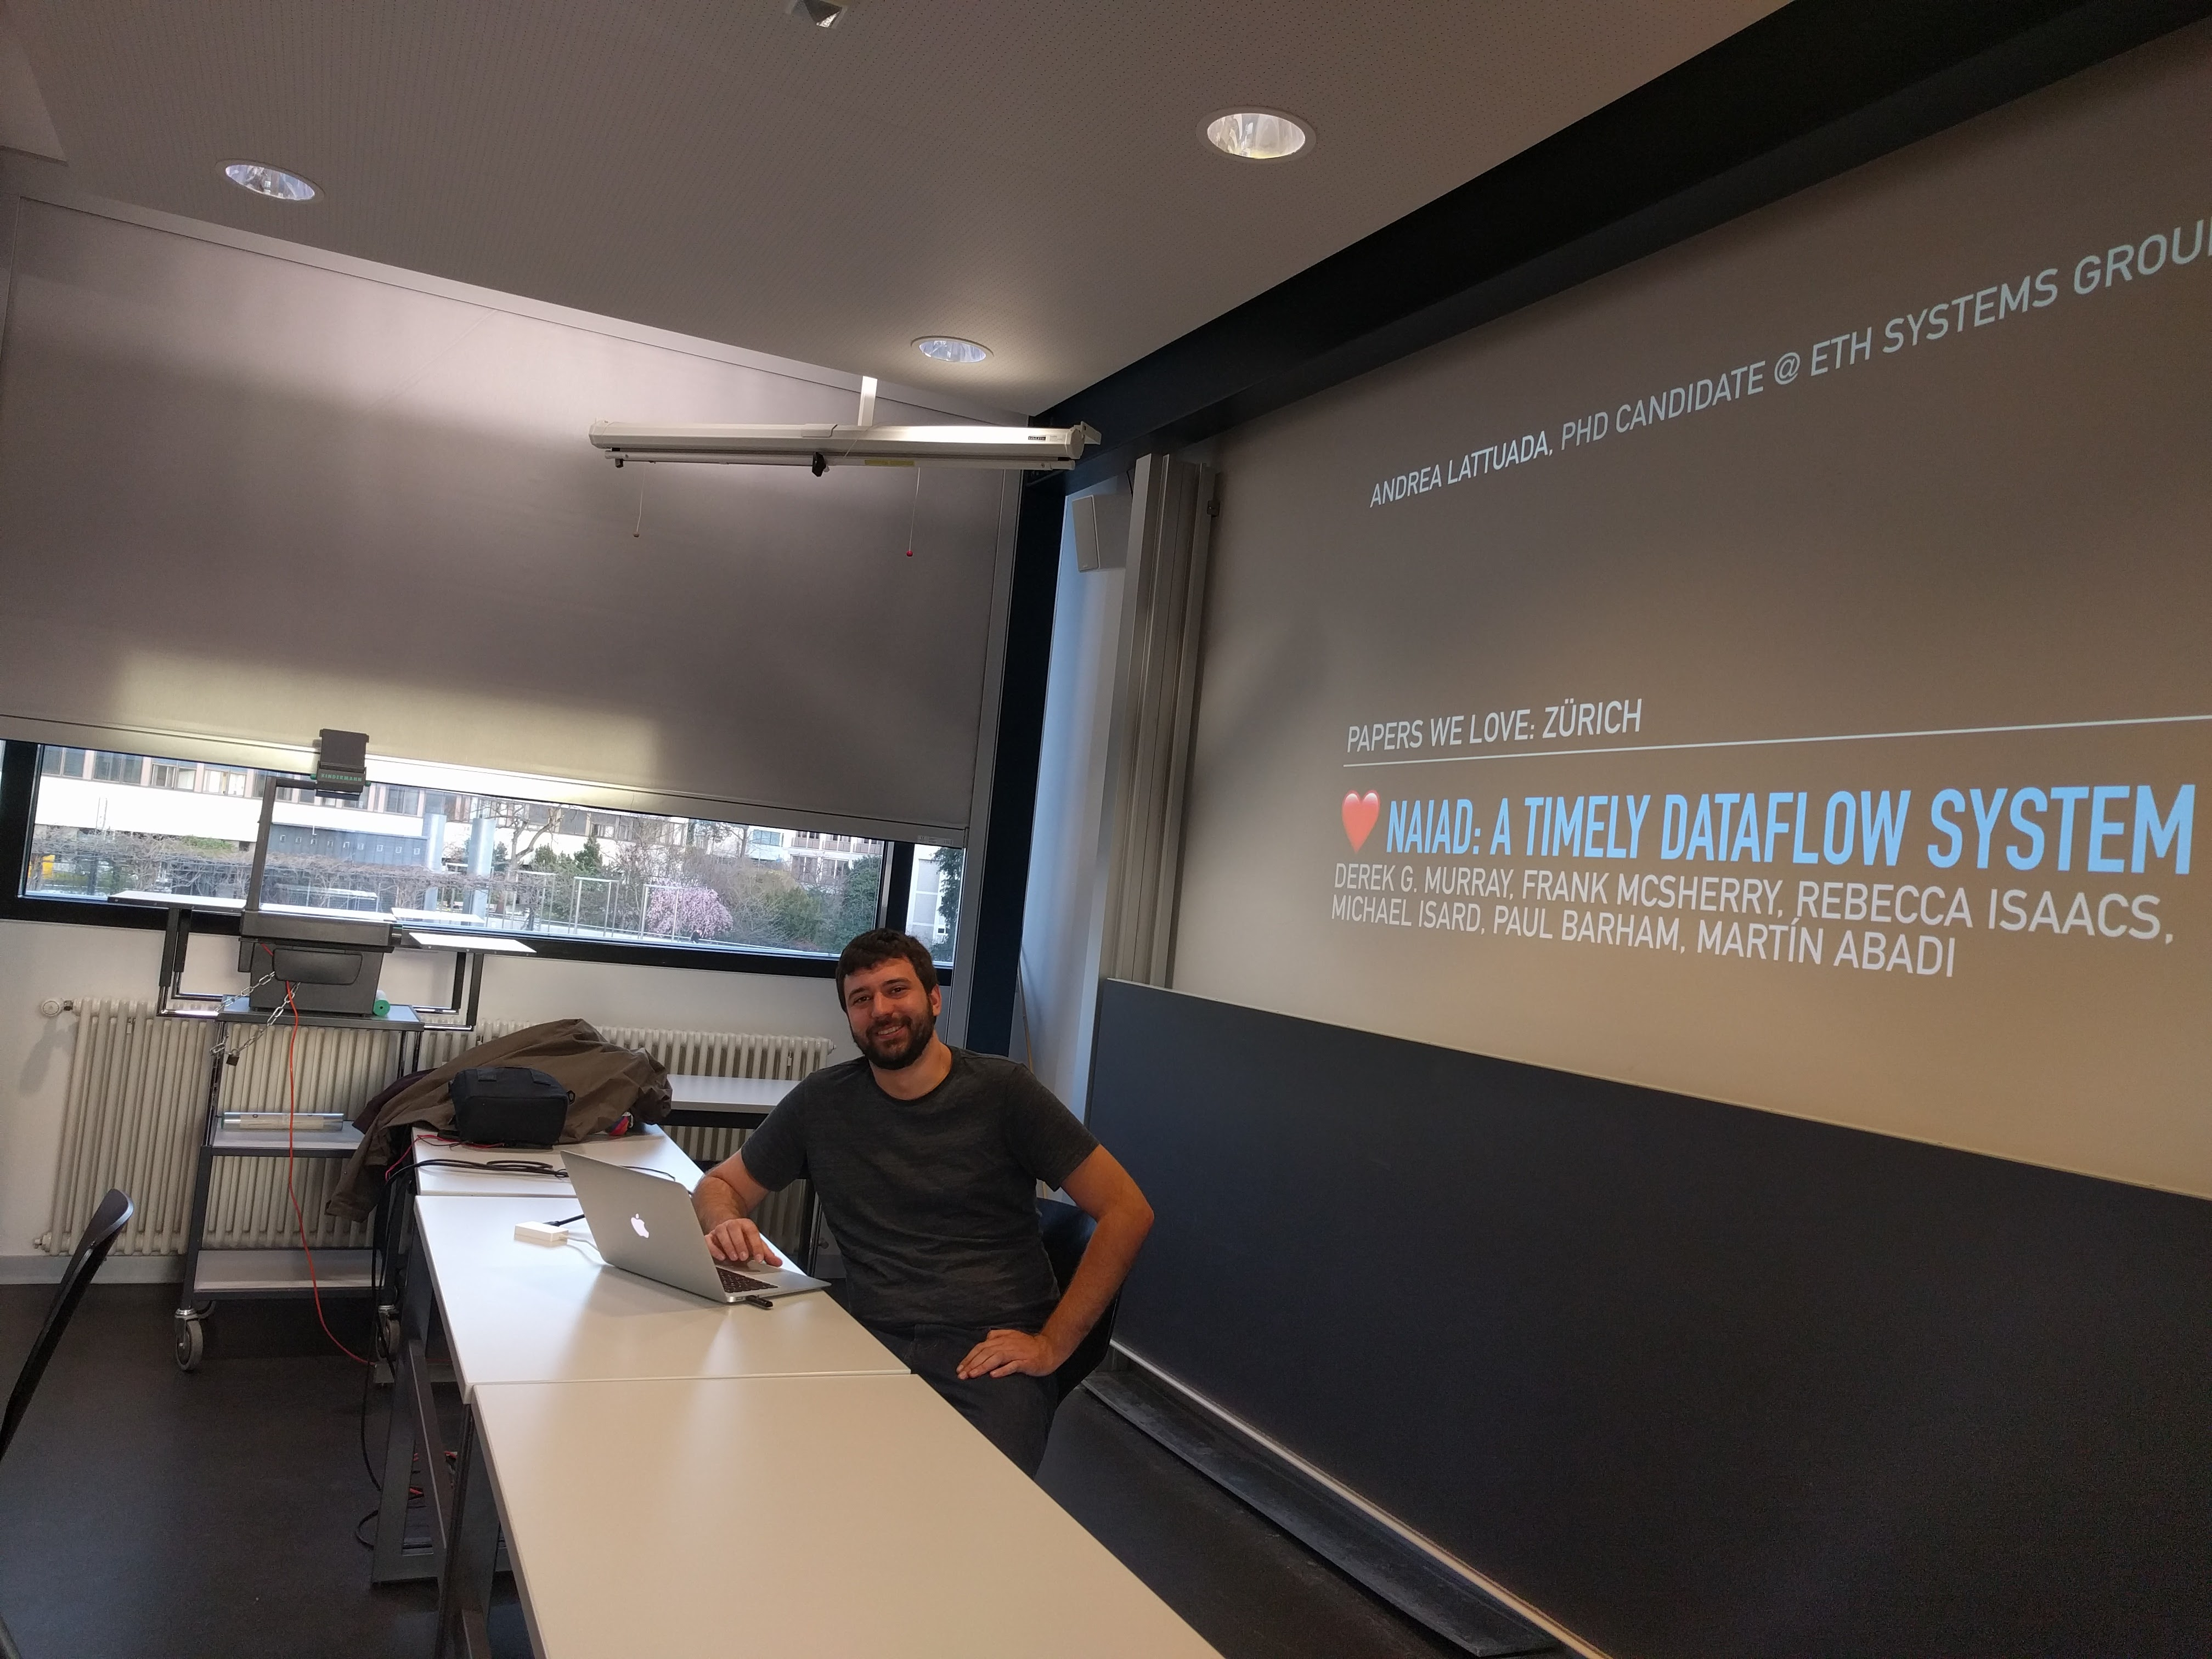
\includegraphics[width=.9\textwidth]{figs/last_time}
	\end{center}
\end{frame}

\begin{frame}{Today: Cilk-5}
\begin{itemize}
    \item A parallel programming language
    \item how to write parallel progrems
    \item how to efficiently execute them
    \item targets single (shared-memory) machines

    \bigskip
    \item original paper written in 1998
\end{itemize}
\end{frame}

\begin{frame}{Why this paper?}{}
\begin{itemize}
\item theory + practice
\item topics: parallel programming, synchronization, languages
\end{itemize}
\end{frame}

\begin{frame}{}
	\begin{center}
	
\includegraphics[width=.9\textwidth]{figs/backtofuture}
    \bigskip

    
\includegraphics[width=.9\textwidth]{figs/back}
	\end{center}
\end{frame}

\begin{frame}{back to 1998...}{}
\centering
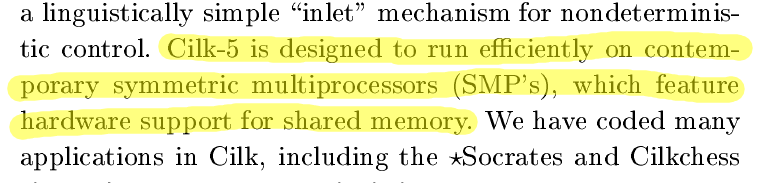
\includegraphics[width=.9\textwidth]{figs/cilk-smp}
\end{frame}

\begin{frame}{back to 1998...}{}
\centering
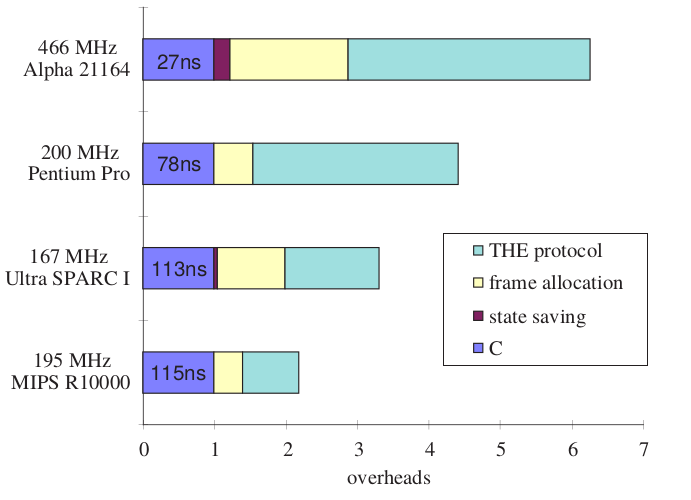
\includegraphics[width=.9\textwidth]{figs/cilk-machines}
\end{frame}

\begin{frame}{back to 1998...}{}
\begin{center}

\includegraphics[width=.4\textwidth]{figs/jiggy}
\end{center}
\end{frame}

\begin{frame}{What followed}{}
  \begin{itemize}
      \item 2006: Intel releases its first dual-core CPU
      \item 2006: Cilk Arts commercializes Cilk
      \item 2008: Cilk++ ships
      \item 2008: Most influential PLDI paper award for 2008
      \item 2009: acquired by Intel
      \item 2010: CilkPlus ships with Intel compiler
      \item 2014: CilkPlus becomes part of gcc ({\ttfamily-fcilk})

      \bigskip
      \item Programming model also picked up by other languages: See Fork/Join
      in Java {\footnotesize
      \url{http://www.oracle.com/technetwork/articles/java/fork-join-422606.html}},
      and OpenMP tasks.
  \end{itemize}
\end{frame}



\begin{frame}[fragile]{Programming model}{}
\begin{itemize}
    \item Task parallelism
    \item Extends C
    \item two basic keywords: {\ttfamily spawn} and {\ttfamily sync}.
\end{itemize}

\begin{columns}
\column{.5\textwidth}
\begin{semiverbatim}
/* Cilk example */
x = \alert{spawn} A();
y = \alert{spawn} B();
C();
\onslide<2->{\alert{sync};
/* x,y are available */}
\end{semiverbatim}
\column{.5\textwidth}
\begin{center}
\begin{tikzpicture}
    \node[spawn-n] (s) {};
    \node[spawn-n,below = 1.3cm] (s1) {};
    \node[fn-n,below right = 1.3cm and 1cm] (a) {\small A};
    \node[fn-n,below right = 2.6cm and 2cm] (b) {\small B};
    \node[fn-n,below = 2.6cm] (c) {\small C};
    \onslide<2->{
        \node[sync-n,below = 4cm] (s3) {};
        \draw[sync-e] (a) -- (s3);
        \draw[sync-e] (b) -- (s3);
        \draw[sync-e] (c) -- (s3);
    }
    \draw[spawn-e] (s) -- (s1);
    \draw[spawn-e] (s) -- (a);
    \draw[spawn-e] (s1) -- (b);
    \draw[spawn-e] (s1) -- (c);
\end{tikzpicture}
\end{center}
\end{columns}
\end{frame}

\begin{frame}[fragile]{Example: run-length encoding (RLE)}{(nope, not fib)}
{
\centering
\Large
\begin{tabular}{ll}
IN:  & {\ttfamily [a,a,a,a,b,b,b,c,c,c,c,c]} \\
OUT: & {\ttfamily [(a,4),(b,3),(c,5)]} \\
\end{tabular}
}
\end{frame}

\begin{frame}[fragile]{Sequential RLE}{(accumulator)}
\begin{semiverbatim}
def rle(xs):
    ret,curr,freq = ([],xs[0],1)
    for item in xs[1:]:
        if item == curr:
            freq += 1
        else:
            ret.append((curr,freq))
            curr,freq = (item,1)
        ret.append((curr,freq))
    return ret
\end{semiverbatim}
\end{frame}

\begin{frame}[fragile]{Recursive \onslide*<2->{parallel }RLE}
\begin{semiverbatim}
def rle_rec(xs):
    if len(xs) <= 1:
        return [(xs[0], 1)]

    mid = len(xs) // 2
    rle1 = \onslide*<2->{\alert{spawn} }rle_rec(xs[:mid])
    rle2 = \onslide*<2->{\alert{spawn} }rle_rec(xs[mid:])
    \onslide*<2->{\alert{sync} }
    return rle_merge(rle1, rle2)

def rle_merge(rle1,rle2):
    if rle1[-1][0] == rle2[0][0]:
        r1, rle1 = rle1[-1], rle1[:-1]
        r2, rle2 = rle2[0], rle2[1:]
        rle1.append((r1[0],r1[1] + r2[1]))
    return rle1 + rle2
\end{semiverbatim}

\onslide<3>{
\begin{tikzpicture}[remember picture,overlay]
    \node[text width=6cm,xshift=-4cm,yshift=-2cm,note] at (current page.north east){
        NOTE: Removing the {\ttfamily spawn} and {\ttfamily sync} keywords results in
        a valid sequential program. In Cilk, this is called the {\bfseries C~elision}.
    };
\end{tikzpicture}
}
\end{frame}

\begin{frame}[fragile]{product using {\ttfamily spawn}/{\ttfamily sync}}{}
\begin{semiverbatim}
{\color{red3}cilk} int product(int *A, int n) \{
  if (n == 1)
    return A[0];
  x1 = {\color{red3}spawn} product(A,n/2);
  x2 = {\color{red3}spawn} product(A+n/2,n-n/2);
  {\color{red3}sync};
  return (x1*x2);
\}
\end{semiverbatim}
\end{frame}

\begin{frame}[fragile]{also: {\ttfamily inlet} and {\ttfamily abort}}{}
\begin{semiverbatim}
cilk int product(int *A, int n) \{
    int p=1;
    {\color{red3}inlet} void mult(int x) \{
        p *= x;
        if (p == 0)
             {\color{red3}abort;}
        return;
    \}
    if (n == 1)
         return A[0];
    mult( spawn product(A, n/2) );
    mult( spawn product(A+n/2, n-n/2) );
    sync;
    return p;
\}
\end{semiverbatim}
\end{frame}

\begin{frame}[fragile]{Executing Cilk programs}{A dynamic graph (tasks, spawns, syncs)}
{\small
\begin{semiverbatim}
\alert{cilk} int fib(int n) \{
     if (n < 2) return (n);
     x = \alert{spawn} fib(n - 1);
     y = \alert{spawn} fib(n - 2);
     \alert{sync};
     return x + y;
\}
\end{semiverbatim}
}

\vspace{-.8cm}
\begin{center}
\begin{tikzpicture}
    %\node[fn-n] (f4) {\footnotesize f(4)};

    \begin{pgfonlayer}{background}
        \node[minimum width=11.5cm, minimum height=4cm] (bg) {};
    \end{pgfonlayer}

    \onslide+<2->{
        \node[spawn-n,below left = 10pt and 1cm of bg.north] (f4-sp1){};
        \node[spawn-n,right=1cm of f4-sp1] (f4-sp2) {};
        \node[sync-n,right=1cm  of f4-sp2] (f4-sy1) {};
    }

    \only<2->{
        \begin{pgfonlayer}{background}
            \node[rectangle,fn-g, fit=(f4-sp1) (f4-sp2) (f4-sy1)] (g4) {};
            \node[right=1pt of g4.west,anchor=east] {\small f(4)};
        \end{pgfonlayer}
    }

    \onslide+<2->{
        \node[spawn-n,below left =1cm and 1cm of f4-sp1] (f43-sp1) {};
        \node[spawn-n,right=1cm of f43-sp1] (f43-sp2) {};
        \node[sync-n,right=1cm  of f43-sp2] (f43-sy1) {};
    }

    \only<2->{
        \begin{pgfonlayer}{background}
            \node[rectangle,fn-g, fit=(f43-sp1) (f43-sp2) (f43-sy1)] (g43) {};
        \end{pgfonlayer}
        \node[right=1pt of g43.west,anchor=east] {\small f(3)};
    }

    \onslide+<2->{
        \node[spawn-n,below right=1cm and 1.5cm of f4-sp2] (f42-sp1) {};
        \node[spawn-n,right=1cm of f42-sp1] (f42-sp2) {};
        \node[sync-n,right=1cm  of f42-sp2] (f42-sy1) {};

    }

    \only<2->{
        \begin{pgfonlayer}{background}
            \node[rectangle,fn-g, fit=(f42-sp1) (f42-sp2) (f42-sy1)] (g42) {};
            \node[right=1pt of g42.west,anchor=east] {\small f(2)};
        \end{pgfonlayer}
    }

    \onslide+<2->{
        \draw[spawn-e] (f4-sp1) -- (f43-sp1);
        \draw[spawn-e] (f4-sp2) -- (f42-sp1);

        \draw[-latex,thick] (f4-sp1) -- (f4-sp2);
        \draw[-latex,thick] (f4-sp2) -- (f4-sy1);
    }

    \onslide+<2->{
        \node[fn-n,below = .5cm of f42-sp1] (f421) {\footnotesize f(1)};
        \node[fn-n,below = .5cm of f42-sp2] (f420) {\footnotesize f(0)};
        \node[spawn-n,below left =.8cm and 2cm of f43-sp1] (f432-sp1) {};
        \node[spawn-n,right=1cm of f432-sp1] (f432-sp2) {};
        \node[sync-n,right=1cm  of f432-sp2] (f432-sy1) {};
    }

    \only<2->{
        \begin{pgfonlayer}{background}
            \node[rectangle,fn-g, fit=(f432-sp1) (f432-sp2) (f432-sy1)] (g432) {};
            \node[right=1pt of g432.west,anchor=east] {\small f(2)};
        \end{pgfonlayer}
    }

    \onslide+<2->{
        \node[fn-n,below right =.6cm and 5pt of f43-sp2] (f431) {\footnotesize f(1)};
        \draw[spawn-e] (f43-sp1) -- (f432-sp1);
        \draw[spawn-e] (f43-sp2) -- (f431);
        \draw[-latex,thick] (f43-sp1) -- (f43-sp2);
        \draw[-latex,thick] (f43-sp2) -- (f43-sy1);

        \draw[spawn-e] (f42-sp1) -- (f421);
        \draw[spawn-e] (f42-sp2) -- (f420);
        \draw[-latex,thick] (f42-sp1) -- (f42-sp2);
        \draw[-latex,thick] (f42-sp2) -- (f42-sy1);
    }

    \onslide+<2->{
        \node[fn-n,below=.5cm of f432-sp1] (f4321) {\footnotesize f(1)};
        \node[fn-n,below=.5cm of f432-sp2] (f4320) {\footnotesize f(0)};
        \draw[spawn-e] (f432-sp1) -- (f4321);
        \draw[spawn-e] (f432-sp2) -- (f4320);
        \draw[-latex,thick] (f432-sp1) -- (f432-sp2);
        \draw[-latex,thick] (f432-sp2) -- (f432-sy1);

    }

    \onslide+<3->{
        \draw[sync-e] (f4321) -- (f432-sy1);
        \draw[sync-e] (f4320) -- (f432-sy1);
    }
    \onslide+<3->{
        \draw[sync-e] (f432-sy1) -- (f43-sy1);
        \draw[sync-e] (f431) -- (f43-sy1);
        \draw[sync-e] (f421) -- (f42-sy1);
        \draw[sync-e] (f420) -- (f42-sy1);
    }

    \onslide+<3->{
        \draw[sync-e] (f43-sy1) -- (f4-sy1);
        \draw[sync-e] (f42-sy1) -- (f4-sy1);

    }
\end{tikzpicture}
\end{center}
\end{frame}

\begin{frame}{How do we efficiently execute Cilk programs?}{}

\begin{quote}
{\bfseries The work-first principle:} \emph{Minimize the scheduling overhead
borne by the \alert<2>{work} of a computation.  Specifically, move overheads out of the
\alert<2>{work} and onto the \alert<2>{critical path}.}
\end{quote}


\bigskip\bigskip
(i.e., make common case fast, push overheads to the rare case)

\end{frame}

\begin{frame}{Performance model}
    \begin{columns}
        \column{.4\textwidth}
        \begin{tikzpicture}[scale=.8,transform shape]
            \node[fn-x] (root) {};
            \node[fn-x,below =1cm of root.center,anchor=center] (o) {};
            \node[fn-x,below left = 1cm and 1cm of o.center,anchor=center] (l) {};
            \node[fn-x,below right = 1.4cm and 2cm of o.center,anchor=center] (r) {};

            \draw[fn-e] (root) -- (o);
            \draw[fn-e] (o) -- (l);
            \draw[fn-e] (o) -- (r);

            \node[fn-x,below left = 1cm and 1cm of l.center,anchor=center] (ll) {};
            \node[fn-x,below right = 1cm and .5cm of l.center,anchor=center] (lr) {};
            \node[fn-x,below left = 1cm and .7cm of lr.center,anchor=center] (lrl) {};
            \node[fn-x,below right = 1cm and .7cm of lr.center,anchor=center] (lrr) {};
            \draw[fn-e] (l) -- (ll);
            \draw[fn-e] (l) -- (lr);
            \draw[fn-e] (lr) -- (lrl);
            \draw[fn-e] (lr) -- (lrr);

            \node[fn-x,below = 2cm of ll.center,anchor=center] (lld)   {};
            \node[fn-x,below = 1cm of lrl.center,anchor=center] (lrld) {};
            \node[fn-x,below = 1cm of lrr.center,anchor=center] (lrrd) {};
            \node[fn-x,below = 1cm of lrld.center,anchor=center] (m) {};
            \node[fn-x,below = 1cm of m.center,anchor=center] (mm) {};

            \draw[fn-e] (ll) -- (lld);
            \draw[fn-e] (lrl) -- (lrld);
            \draw[fn-e] (lrr) -- (lrrd);
            \draw[fn-e] (lld) -- (m);
            \draw[fn-e] (lrld) -- (m);
            \draw[fn-e] (lrrd) -- (m);
            \draw[fn-e] (m) -- (mm);

            \node[fn-x,below right = 1cm and 1cm of r.center,anchor=center] (rr)   {};
            \node[fn-x,below left = 1cm and 1cm of r.center,anchor=center] (rl)   {};
            \node[fn-x,below = 2.1cm of rl.center,anchor=center] (rld)   {};
            \node[fn-x,below = 1cm of rr.center,anchor=center] (rrd)   {};

            \draw[fn-e] (r) -- (rl);
            \draw[fn-e] (r) -- (rr);
            \draw[fn-e] (rr) -- (rrd);
            \draw[fn-e] (rl) -- (rld);

            \node[fn-x,below right = .2cm and 2.5cm of mm.center,anchor=center] (mmm)   {};

            \draw[fn-e] (rrd) -- (mmm);
            \draw[fn-e] (rld) -- (mmm);
            \draw[fn-e] (mm) -- (mmm);

            \onslide<2>{
                \foreach \n in {root,o,l,r,ll,lr,lrl,lrr,lld,lrld,lrrd,m,mm,rr,rl,rld,rrd,mmm}
                    \node[fn-x,fill=red3] at (\n) {};
            }

            \onslide<3>{
                \foreach \n in {root,o,l,lr,lrl,lrld, m,mm,mmm}
                    \node[fn-x,fill=red3] at (\n) {};
            }
        \end{tikzpicture}

    \column{.6\textwidth}
        \begin{sItemize}
            \item     $T_p$: Execution time on P CPUs
            \medskip

            \item<2-> $T_1$: {\bfseries work} \\
            {\small (Execution time for all nodes)}
            \item<3-> $T_\infty$: {\bfseries span} / {\bfseries critical path} \\
            {\small (Execution time for $\infty$ CPUs)}

            \bigskip \bigskip
            \item<4-> work-first: move overheads to $T_\infty$

        \end{sItemize}

    \end{columns}
\end{frame}

\begin{frame}{Scheduiling tasks}{}
\begin{center}
\begin{tikzpicture}
\begin{scope}[every node/.style={minimum width=1cm,minimum height=15pt,rectangle,draw}]
    \begin{scope}[start chain=going above,node distance=0pt]
    \node[on chain,draw=none] (p0) {$P_0$};
    \foreach \i in {1,...,5}
        \node[on chain,draw] (n0-\i) {};

    \node[on chain,draw=none,right=2cm] at (p0) (p1) {$P_1$};
    \foreach \i in {1,...,5}
        \node[on chain,draw] (n1-\i) {};

    \node[on chain,draw=none,right=2cm] at (p1) (p2) {$P_2$};
    \foreach \i in {1,...,5}
        \node[on chain,draw] (n2-\i) {};

    \node[on chain,draw=none,right=2cm] at (p2) (p3) {$P_3$};
    \foreach \i in {1,...,5}
        \node[on chain,draw] (n3-\i) {};
    \end{scope}

    \node[rectangle,fill=none,draw=none,anchor=center] at (n0-1) {\footnotesize $T_0$};
    \node[rectangle,fill=none,draw=none,anchor=center] at (n0-2) {\footnotesize $T_1$};
    \node[rectangle,fill=none,draw=none,anchor=center] at (n0-3) (t2) {\footnotesize $T_2$};
    \node[rectangle,fill=none,draw=none,anchor=center] at (n1-1) {\footnotesize $T_3$};
    \node[rectangle,fill=none,draw=none,anchor=center] at (n1-2) {\footnotesize $T_4$};
    \node[rectangle,fill=none,draw=none,anchor=center] at (n3-1) {\footnotesize $T_5$};
    \node[rectangle,fill=none,draw=none,anchor=center] at (n3-2) {\footnotesize $T_6$};

    \onslide<2> {
        \draw[-latex,ultra thick,red] ($ (t2.center) + (0,-0.1)$) to[out=-90,in=180]
               ++(1.3,-.5) node[inner sep=1,draw=none,fill=white]
               {\bfseries\large spawn} to[out=0,in=180] (n2-1.west);
    }
    \onslide<3-> {
        \draw[-latex,ultra thick,red] ($ (p2) + (-0.3,0)$) to[out=-90,in=180]
               ++(-1.3,-.3) node[inner sep=1,draw=none,fill=white]
               {\bfseries\large steal} to[out=180,in=0] (n0-1.east);
    }
\end{scope}
\end{tikzpicture}
\end{center}

\begin{overlayarea}{\textwidth}{4.4cm}
\onslide*<2> {
    {\bfseries work sharing:} when new tasks are created, scheduler
    tries to send them to inactive CPUs
}
\onslide+<3->{%
{\bfseries work stealing:} Idle processors try to steal tasks
\begin{itemize}
    \item child executes first
    \item tasks are stolen from the bottom
    \item intuitively similar to DFS (good space properties)
    \item where do we steal from? \onslide<4->{\bfseries randomly choose}
\end{itemize}
}
\end{overlayarea}
\end{frame}

\begin{frame}{Cilk's work-stealing scheduler}

    \begin{itemize}
        \item $T_p = T_1 / P + \mathcal{O}(T_\infty)$ \\
        \begin{itemize}
            \item[-] {\small ($T_1 / P$ and $T_\infty$ are lower bounds)}
        \end{itemize}
        \bigskip
        \item requires $S_p \leq P S_1$ stack space
    \end{itemize}

    \vfill
    see: Scheduling Multithreaded Computations by Work Stealing, by Blumofe and
    Leiserson.
\end{frame}

\begin{frame}{Parallel slackness}{Cilk's basic assumption}
    \begin{itemize}
        \item program parallelism $T_1 /  T_\infty$
        \item machine parallelism $P$

        \bigskip
        \item $P \ll T_1 / T_\infty$
        \item parallel slack: $\left( T_1 /  T_\infty \right) / P$
        \medskip

        \begin{equation*}
           \left.%
           \begin{aligned}
           T_p     &=   T_1 / P + \mathcal{O}(T_\infty) \\
           T_1 / P &\gg T_\infty \\
           \end{aligned}%
           \qquad
           \right \} \Rightarrow T_p \approx T_1 / P \qquad \text{\small(linear speedup)}
         \end{equation*}

        \medskip
        \item Intiuitively:
        \begin{itemize}
            \item[+] program does not depend on number of CPUs
            \item[+] allows better load balancing
        \end{itemize}

    \end{itemize}
\end{frame}

\begin{frame}{Parallel slackness $\Rightarrow$ work-first principle}

\begin{eqnarray*}
            T_p &\approx& T_1 / P \\
            c_1 = T_1/T_s \Rightarrow T_p &\approx& c_1 T_s / P \qquad \text{\small $T_s$: time of C elision} \\
\end{eqnarray*}

\begin{itemize}
    \item[] principle: minimize $c_1$ even at the expanse of $c_\infty$
    \item[] (yet, this has limits -- authors' discussion on Cilk-4)
\end{itemize}

\end{frame}

\begin{frame}{Compilation strategy}{}
Two versions of each Cilk function (task)
\begin{itemize}
    \item fast version
    \begin{itemize}
        \item invariant: never stolen
        \item as close to C elision as possible
    \end{itemize}

    \item slow version
    \begin{itemize}
        \item when a task is stolen, slow version is executed on thief processor
        \item needs to restore state
    \end{itemize}

    \item Original implementation: cilk2c translation
\end{itemize}
\end{frame}

\begin{frame}[fragile]{C elision}{Only use the execution stack}
\begin{semiverbatim}{\small
f(n) \{
    // spawn f(n-1)
    x = f(n-1);
    // spawn f(n-2)
    y = f(n-2);
    // sync
    return x + y;
\}
}\end{semiverbatim}
%\begin{tikzpicture}[]
%\node[fn-inact,minimum height=5cm,label=above:stack] (s) {};
%\node<1-7>[fn-activ,anchor=north] at (s.north) (f3) {f(3)};
%\node<1-6>[fn-activ,anchor=north] at (f3.south) (f2) {f(2)};
%\node<2>[fn-activ,anchor=north] at (f2.south) {f(1)};
%\node<4>[fn-activ,anchor=north] at (f2.south) {f(0)};
%\end{tikzpicture}
\end{frame}

\begin{frame}{Cactus stack}{}
\begin{columns}
\column{.3\textwidth}
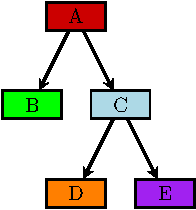
\includegraphics[width=\textwidth]{figs/cilk-cactus-spawn}
\column{.7\textwidth}
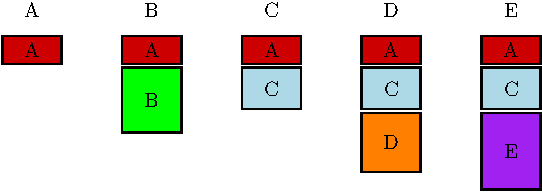
\includegraphics[width=\textwidth]{figs/cilk-cactus-stack}
\end{columns}
\end{frame}

\begin{frame}[fragile]{Cilk fast version}{use the execution stack, record state}
\begin{semiverbatim}{\small
f(n) \{
    frame = alloc_frame();
    // spawn f(n-1)
    frame->entry = 1;
    frame->n = n;
    push(frame);
    x = f(n-1);
    frame = pop();
    if (!frame)
      return STOLEN;
    // spawn f(n-2)
    ...
    // sync
    free_frame(frame)
    return x + y;
\}
}\end{semiverbatim}
\end{frame}


\begin{frame}[fragile]{Cilk slow version}{restore state, sync}
\begin{semiverbatim}{\small
f_slow(frame) \{
    switch (frame->entry) \{
        case 1: goto a;
        ...
    \}
    // spawn f(n-1)
    ... (same as fast version) ...
    if (0) \{ a: n = frame->n; \}
    // spawn f(n-2)
    ... (same as fast version) ...
    // sync
    wait_for_children();
    free_frame(frame)
    return frame->x + frame->y;
\}}
\end{semiverbatim}
\end{frame}


\begin{frame}{worker/thief synchronization}{}
\begin{itemize}
    \item basic scheduler data structure: double-ended queue (\emph{deque})
    \item worker: operates on {\bfseries T}ail: push / pop
    \item thief: operates on {\bfseries H}ead: steal

    \medskip
    \item traditional approach: lock for accessing deque
    \begin{itemize}
        \item adds overhead to worker!
    \end{itemize}
\end{itemize}
\end{frame}

\begin{frame}{TH(E) protocol}{}
	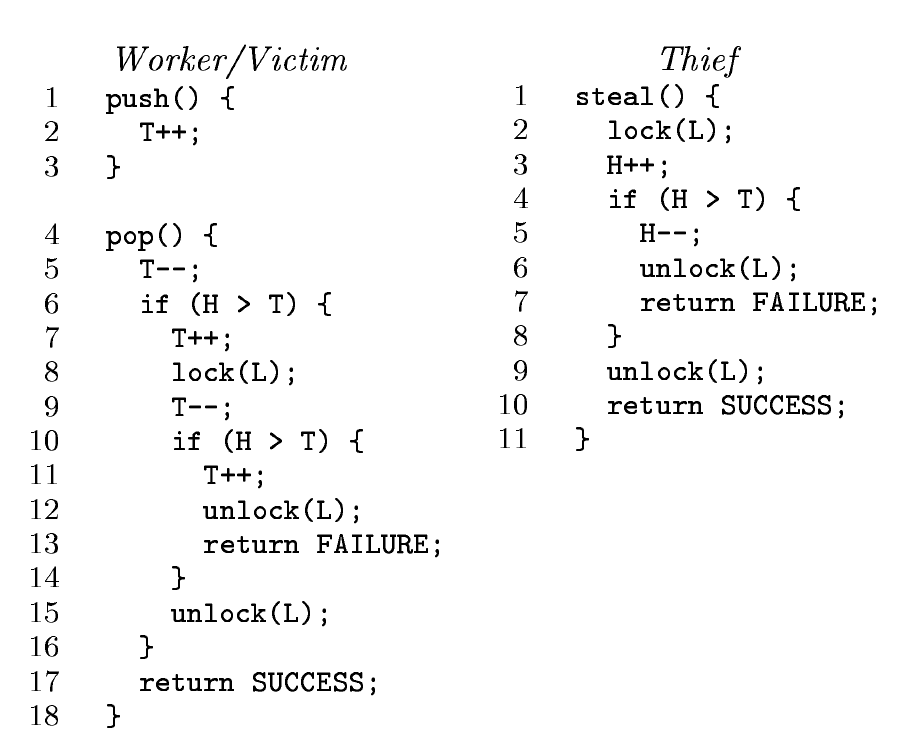
\includegraphics[width=.9\textwidth]{figs/simplified-the}
\end{frame}

\begin{frame}[fragile]{Note \#1: improving performance}{}

\begin{semiverbatim}
def rle_rec(xs):
    if len(xs) <= cutoff:
        return rle(xs)
    mid = len(xs) // 2
    rle1 = spawn rle_rec(xs[mid:])
    rle2 = spawn rle_rec(xs[:mid])
    sync
    return rle_merge(rle1, rle2)
\end{semiverbatim}
\end{frame}

\begin{frame}{Note \#2: data structures}{}
\begin{itemize}
    \item efficient partition and concatation
    \item lists: poor partition
    \item arrays: poor concatation

    \medskip
    \item Ropes: an Alternative to Strings\\
    Boehm et al. (1995)
    \item Skip lists: a probabilistic alternative to balanced trees\\
    Pugh (1990)
    \item implementation: \url{https://github.com/kkourt/xarray}
\end{itemize}
\end{frame}

\begin{frame}[fragile]{Note \#3: data vs task parallelism}{}

\begin{semiverbatim}{\large
reduce(rle_merge, map(lambda x: [(x,1)], input))
}\end{semiverbatim}

\begin{itemize}
    \item[] ({\ttfamily rle\_merge} is an associative operation)
\end{itemize}
\end{frame}


\begin{frame}{}{}

\begin{center}
\LARGE
Thank you!

\bigskip
Qs? Pizza?
\end{center}
\end{frame}

\end{document}
